\documentclass{article}
\usepackage[margin=1in]{geometry}
\usepackage{graphicx}
\usepackage{xcolor}
\usepackage{float}
\usepackage{amsmath}
\usepackage{cite}
\usepackage{hyperref}
\usepackage{indentfirst}
\graphicspath{{..} {./images}}

\definecolor{navy-blue}{rgb}{0.22,0.38,0.71}

\renewcommand{\contentsname}{\vspace*{-2\baselineskip}}

\hypersetup{
	colorlinks,
	linkcolor=black,
	urlcolor=blue,
	citecolor=black
}
  		
\begin{document}
\begin{titlepage}
	\centering
	{\huge Lab 4 - Analog Modulation with SDR}\\[0.25 in]
	
\includegraphics[width=0.6\textwidth]{ua_logo.png}\\[0.25 in]
	{\large \textbf{ECE 531 - Software Defined Radio\\[0.25 in]
	March 21, 2025\\[0.25 in]}}
	{\large Owen Sowatzke, osowatzke@arizona.edu\\[0.05 in]
	Department of Electrical \& Computer Engineering\\[0.05 in]
	University of Arizona, Tucson, AZ 85721\\[0.5 in]}
	\hypersetup{linkcolor=navy-blue}
	\noindent\hrulefill
	\tableofcontents
	\noindent\hrulefill
\end{titlepage}

% \setlength{\parindent}{0pt}

\section{Introduction}
%Introduction to the laboratory experiment, including a brief description of the objectives and goals.

In this lab, we perform analog demodulation with GNU Radio. We specifically concentrate on FM demodulation, because the AM radio band (530 kHz - 1700 kHz) lies outside of the PlutoSDR's operating frequency (70 MHz - 6 GHz). We start by demodulating FM radio signals in GNU radio using the built-in FM demodulation block. Then, we perform FM demodulation with a custom demodulation block. We perform multiple experiments to analyze each of our flowcharts. In the work that follows, we present the procedures and results for each of these experiments. Finally, even though we cannot demodulate AM radio signals with the PlutoSDR, we discuss the process for doing so in GNU radio.  

\section{Procedure}
% Detailed explanation of the laboratory experiment, including the design, implementation, and testing of the system.

In this section, we provide the procedures for each of our experiments. We start by evaluating FM demodulation with GNU Radio's built-in FM demodulation block. Then, we perform manual demodulation using a custom demodulation block. In each flowchart, we analyze the use of resampling blocks. Then, we analyze the spectrum and audio quality of the resulting signals.

\subsection{FM Demodulation using GNU Radio}
\label{section::fm_demod_gnu_radio}

In this experiment, we use the GNU radio flowchart shown in Figure \ref{fig::fm_radio_flowchart} to perform FM demodulation.

\begin{figure}[H]
	\centerline{\fbox{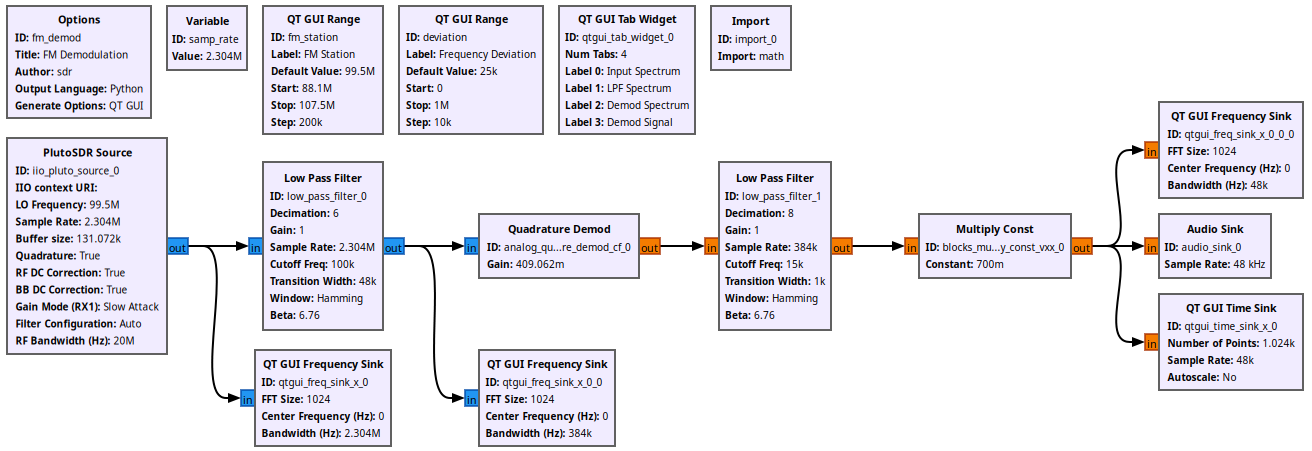
\includegraphics[width=0.7\textwidth]{fm_radio_flowchart.png}}}
	\caption{Flowchart for FM Demodulation}
	\label{fig::fm_radio_flowchart}
\end{figure}

\noindent Using the flowchart, we capture images of the spectrum before and and after demodulation. We also turn on averaging to reduce the variance of the noise floor. This allows us to better visualize the FM spectrum. Next, we list the decimation blocks in the flowchart and explain why they are needed. Then, we discuss when a rational resampler block is needed and why it is not needed for the flowchart shown in Figure \ref{fig::fm_radio_flowchart}. Using the flowchart, we analyze the quality of the audio output and describe what modifications can be made to improve the audio quality. Finally, we justify the 100 kHz cutoff frequency of the low-pass filter (LPF).

\subsection{Manual RF Demodulation}

In this experiment, we repeat the analysis from Section \ref{section::fm_demod_gnu_radio} using a quadrature demodulator and low-pass filter instead of an FM demodulator block. Using the flowchart, we specifically capture images of the spectrum before and after demodulation. We also enable spectral averaging as we did above. Next, we examine the role of decimation, interpolation, and resampling blocks in our flowchart. Then, we compare the audio quality with custom demodulation blocks to the audio quality of the flowchart shown in Figure \ref{fig::fm_radio_flowchart}. Finally, we describe how we might improve the audio quality.

\section{Results}
% Results and discussion of the laboratory experiment, including captured outputs, observations, and responses to laboratory questions.

In this section, we analyze the results of our experiments. First, we analyze the performance of the built-in FM demodulation block, concentrating on the spectrum, resampling blocks, and audio quality. Then, we perform similar analysis using a custom demodulation block, composed of a quadrature demodulation block and a low-pass filter.

\subsection{FM Demodulation using GNU Radio}

In this section, we use the flowchart shown in Figure \ref{fig::fm_radio_flowchart} to receive, demodulate, and play audio from FM radio signals. We specifically tune the flowchart to 99.5 MHz (99.5 FM) and capture the spectrum before and after demodulation. The input spectrum is captured in Figure \ref{fig::fm_radio_input_spectrum}.

\begin{figure}[H]
	\centerline{\fbox{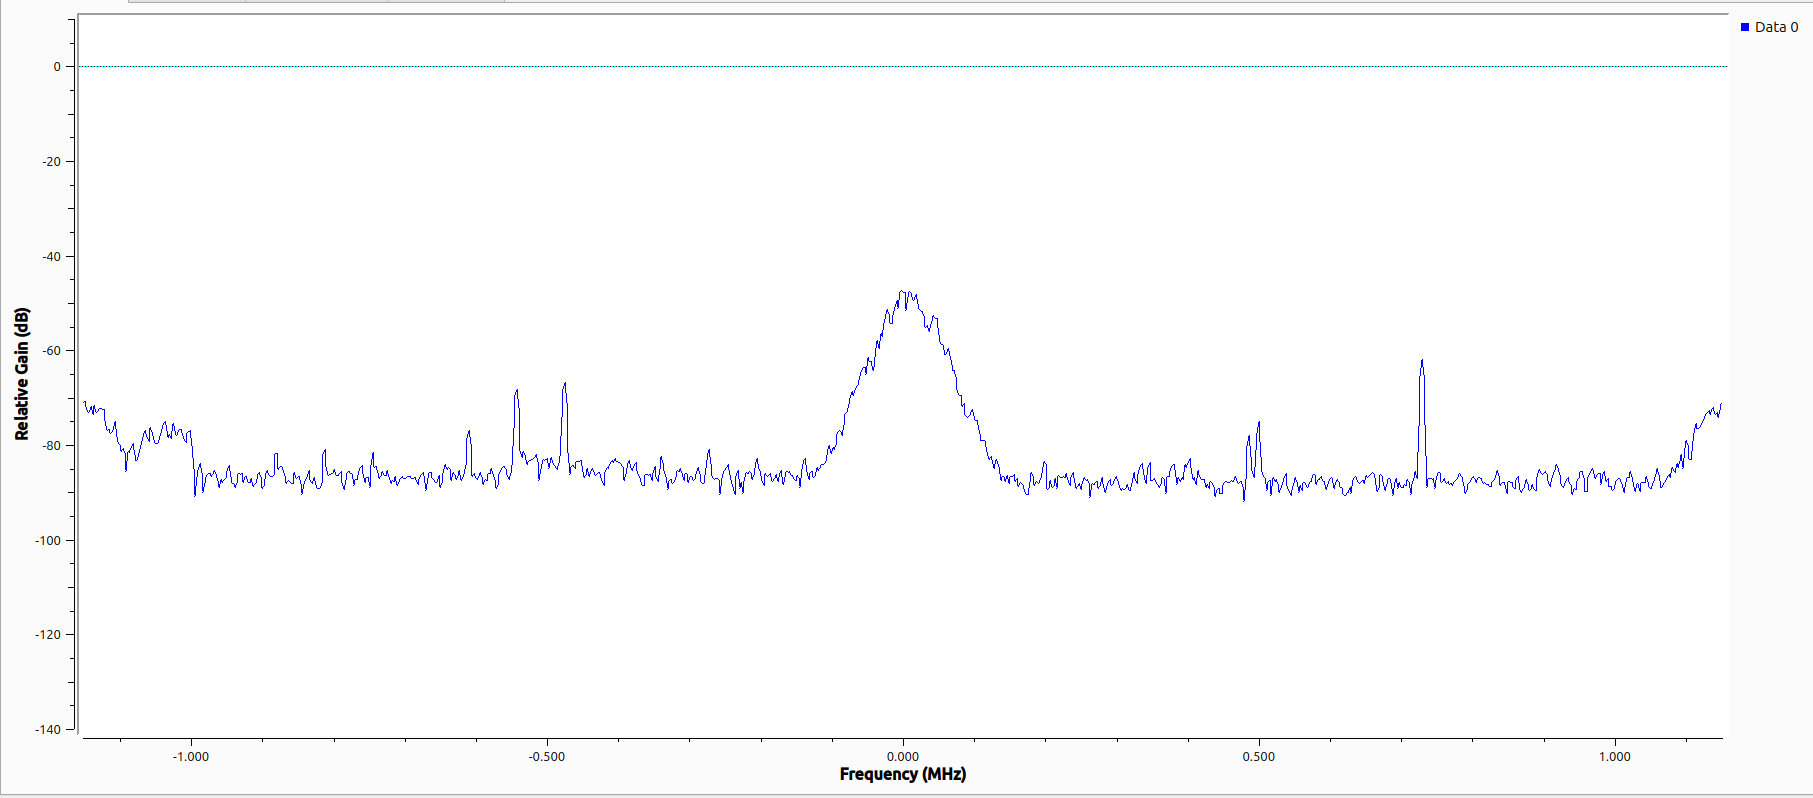
\includegraphics[width=0.7\textwidth]{fm_radio_input_spectrum.png}}}
	\caption{FM Radio Input Spectrum}
	\label{fig::fm_radio_input_spectrum}
\end{figure}

\noindent Looking at the input spectrum, we see that FM radio signal is centered at the middle of the band. We also see that the signal is sampled at a rate higher than the input bandwidth. Next, we analyze the spectrum after the LPF and decimate by 6. The resulting spectrum is shown in Figure \ref{fig::fm_radio_lpf_spectrum}.

\begin{figure}[H]
	\centerline{\fbox{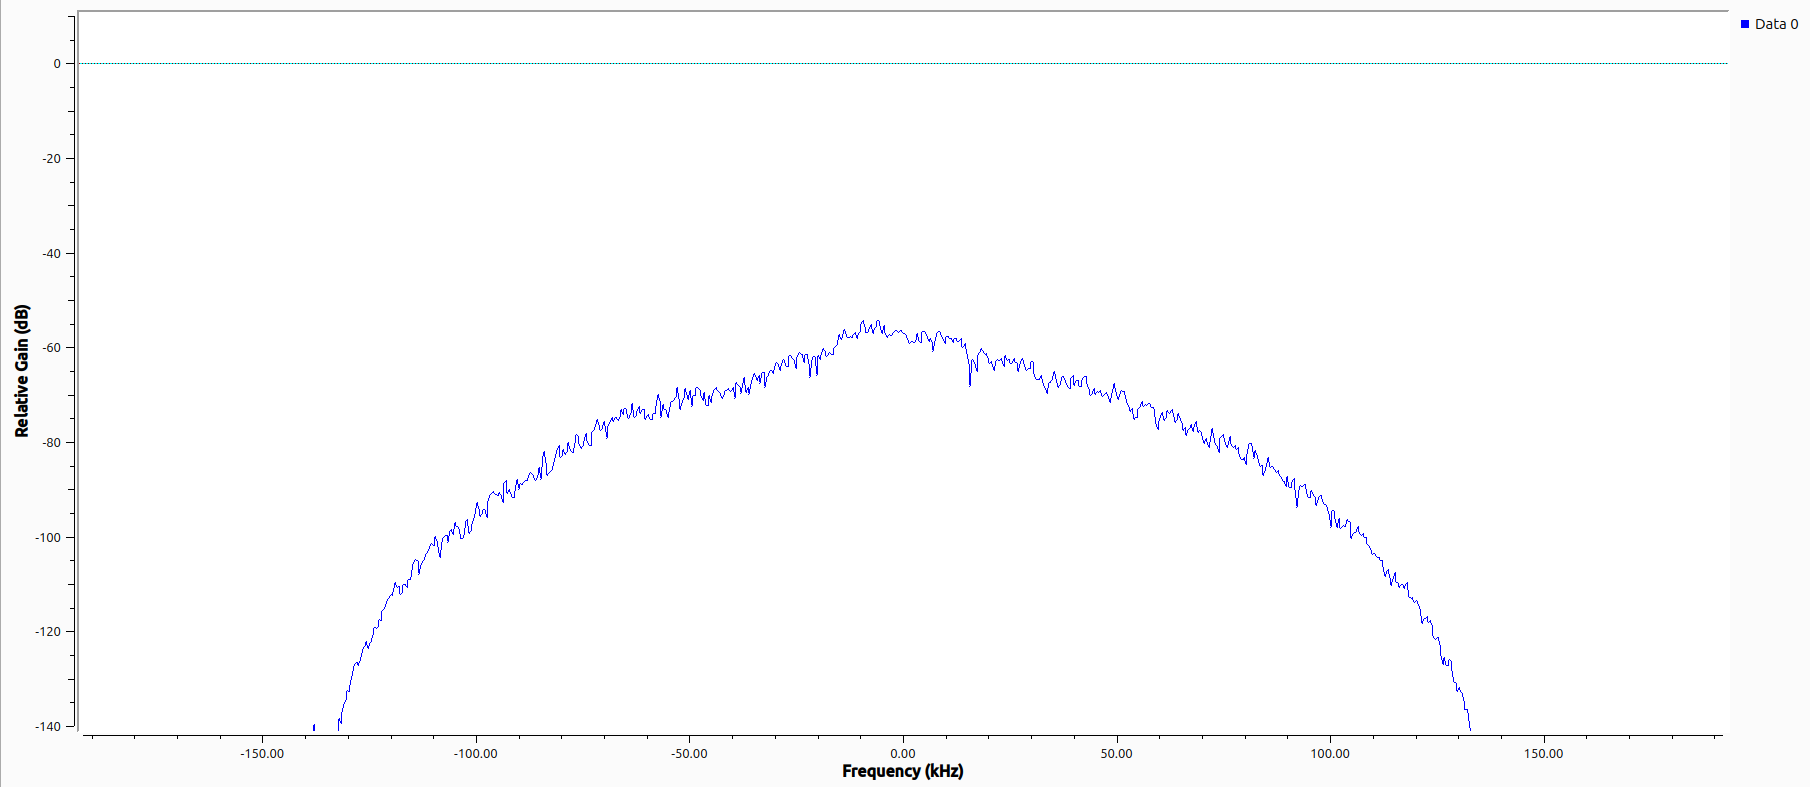
\includegraphics[width=0.7\textwidth]{fm_radio_lpf_spectrum.png}}}
	\caption{FM Radio LPF Spectrum}
	\label{fig::fm_radio_lpf_spectrum}
\end{figure}

\noindent Examining the low pass filter output, we see that we have passed most of the FM radio spectrum. We also see that we have properly band-limited our signal to prevent aliasing during decimation. Finally, we examine the spectrum of the demodulated signal, which is shown in Figure \ref{fig::fm_radio_demod_spectrum}.

\begin{figure}[H]
	\centerline{\fbox{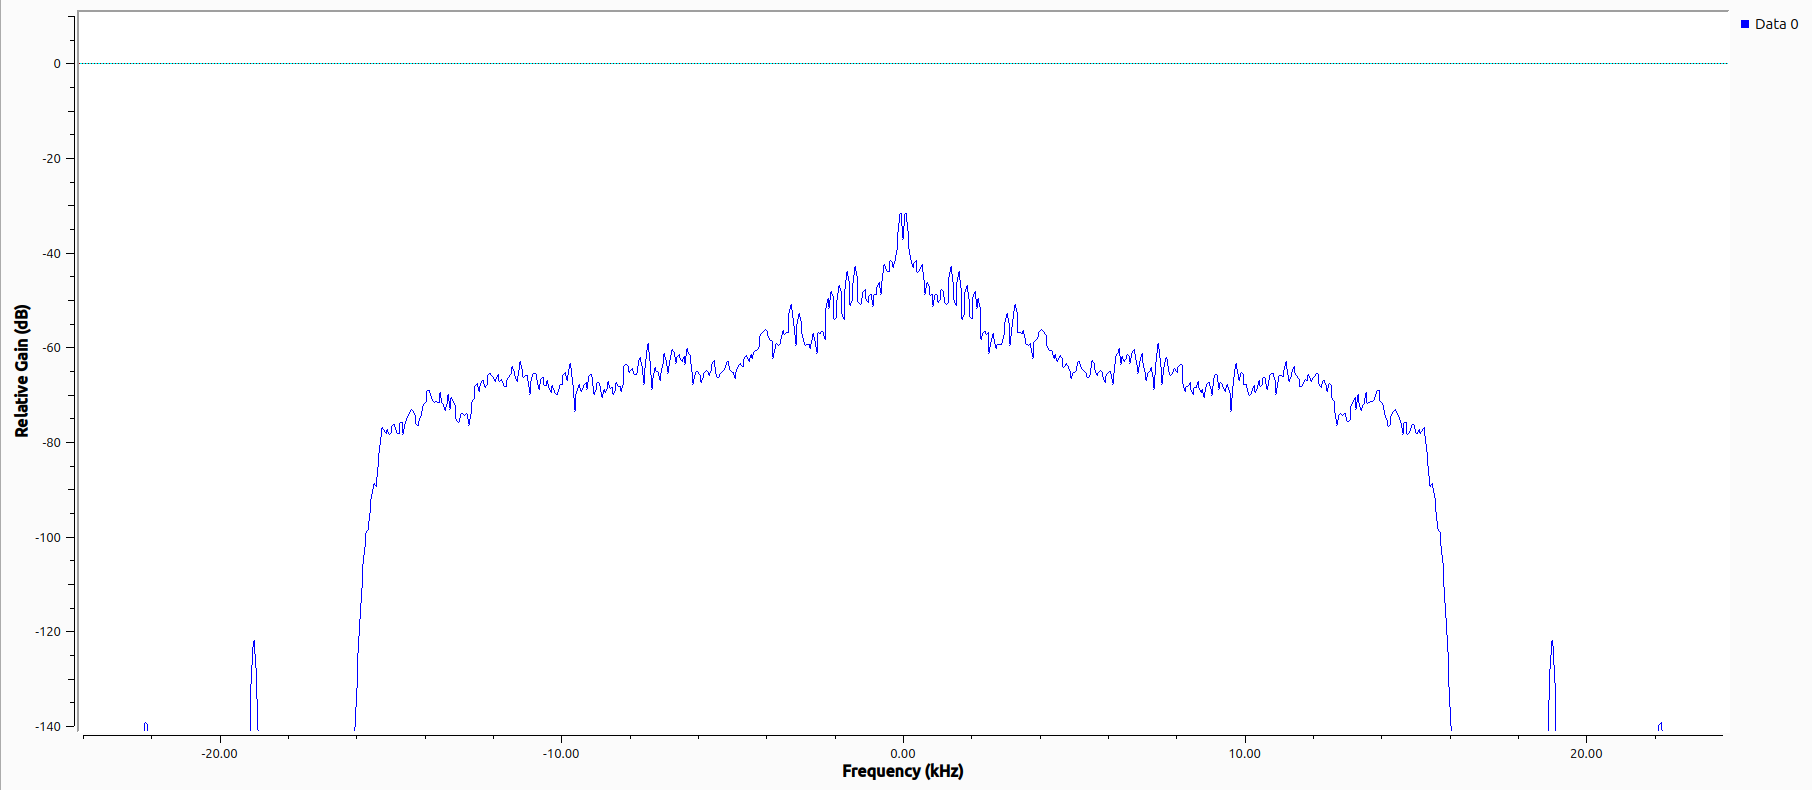
\includegraphics[width=0.7\textwidth]{fm_radio_demod_spectrum.png}}}
	\caption{Demodulated FM Signal Spectrum}
	\label{fig::fm_radio_demod_spectrum}
\end{figure}

\noindent Note that the spectrum of the demodulated signal is very different than the input spectrum. This is because the demodulation block computes the phase difference between adjacent samples and filters the resulting signal. Note that the filter cutoff frequency is approximately 15 kHz, which is sufficient for audio signals. The filtering also prevents aliasing when we decimate the signal to the 48 kHz audio output rate.

As hinted at above, there are two decimating filters within the block diagram. One is before the FM demodulation block and limits the bandwidth of the signal to the width of the RF channel. The second filter is included with the FM demodulation block, and it limits the frequency of the audio output for the audio sink. The first filter includes a decimate by 6, and the second filter includes a decimate by 8. As a result, our sample rate falls from 2.304 MHz to 48 kHz. Note that this decimation is important because we must feed the audio source at a rate of 48 kHz.

In the flowchart, a rational resampler block is needed instead of decimating FIRs if the input sampling rate is not a multiple of the audio sink sampling rate. In Figure \ref{fig::fm_radio_flowchart}, the input sampling rate is a multiple of the audio sink sampling rate (i.e. $48\ \text{kHz} \times 48 = 2.304\ \text{MHz}$). Therefore, a rational resampler block is not needed.

The FM radio sound quality from our flowchart is pretty good. However, we can improve the SNR of our signal, by decreasing the RF bandwidth. Our initial RF bandwidth of 20 MHz is larger than the sampling rate of 2.304 MHz, which allows some spectral content to alias. FM radio channels have a bandwidth of 200 kHz, so we want a sample rate larger than 200 kHz and less than the sampling rate of 2.304 MHz. The RF filter is not perfect, so we should choose a bandwidth in the middle of this range to minimize ripple across the passband and minimize out-of-band aliasing. The 100 kHz cutoff frequency for the low-pass filter (LPF) is chosen to match the 200 kHz bandwidth of the FM radio signal instead of the LPF sampling rate. Because the filter bandwidth is less than the sampling rate, we will not have problems with aliasing. Additionally, the reduced bandwidth fully captures our signal, while reducing the amount of noise entering the FM demodulator.

\subsection{Manual RF Demodulation}

In this section, we perform FM radio demodulation without using the built-in FM demodulation block. We instead use the Quadrature demodulation followed by a low-pass filter. Our resulting flowchart is shown in Figure \ref{fig::fm_radio_user_flowchart}.

\begin{figure}[H]
	\centerline{\fbox{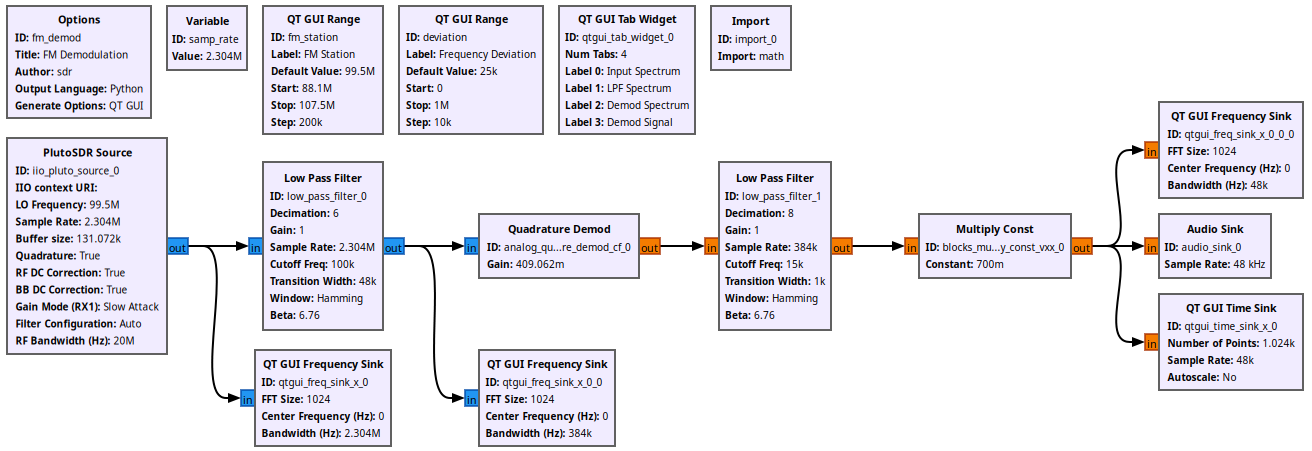
\includegraphics[width=0.7\textwidth]{fm_radio_user_flowchart.png}}}
	\caption{FM Radio Flowchart with Custom Blocks}
	\label{fig::fm_radio_user_flowchart}
\end{figure}

\noindent In this flowchart, the quadrature demodulation block computes the phase difference between adjacent samples, which is an instantaneous measurement of the frequency. This phase difference is then scaled to produce an amplitude in range $[0, 1)$. The phase difference between adjacent samples is then passed through a low-pass filter to limit to frequency of the output signal to $\pm 15\ \text{kHZ}$. The low-pass filter also decimates the signal to get to the audio rate of 48 kHZ.

As we did above, we look at the spectrum of the signal before and after demodulation. Figure \ref{fig::fm_radio_user_input_spectrum}, shows the spectrum of the received FM radio signal.
 
\begin{figure}[H]
	\centerline{\fbox{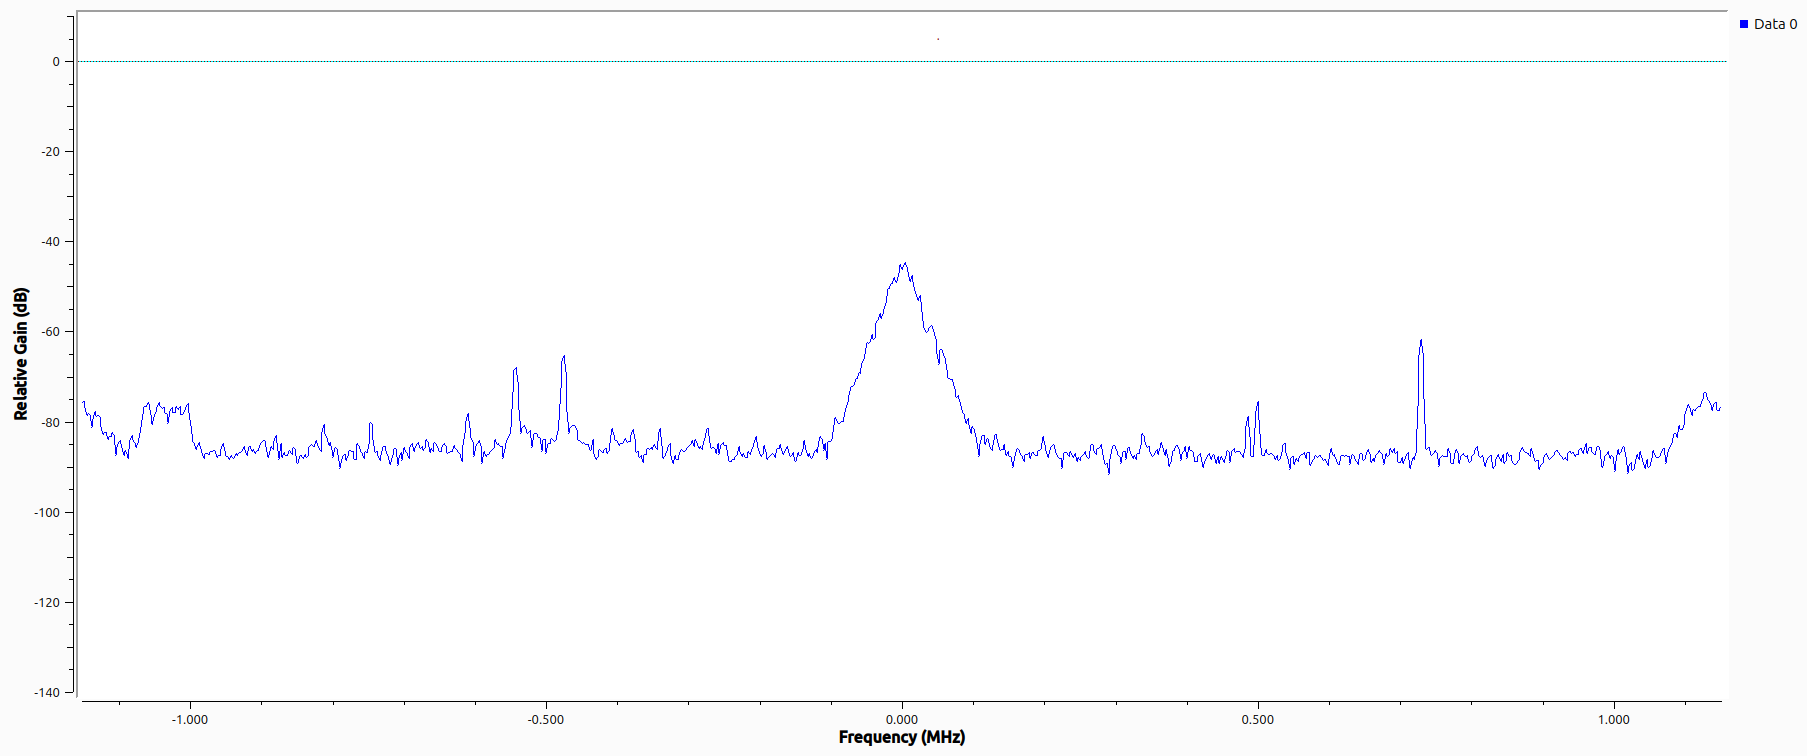
\includegraphics[width=0.7\textwidth]{fm_radio_user_input_spectrum.png}}}
	\caption{FM Radio Input Spectrum}
	\label{fig::fm_radio_user_input_spectrum}
\end{figure}

\noindent Note the input spectrum is identical to what was shown in Figure \ref{fig::fm_radio_input_spectrum} because the flowchart through this point is the same.  We also attach the spectrum at the output of the low-pass filter, which is shown in Figure \ref{fig::fm_radio_user_lpf_spectrum}.

\begin{figure}[H]
	\centerline{\fbox{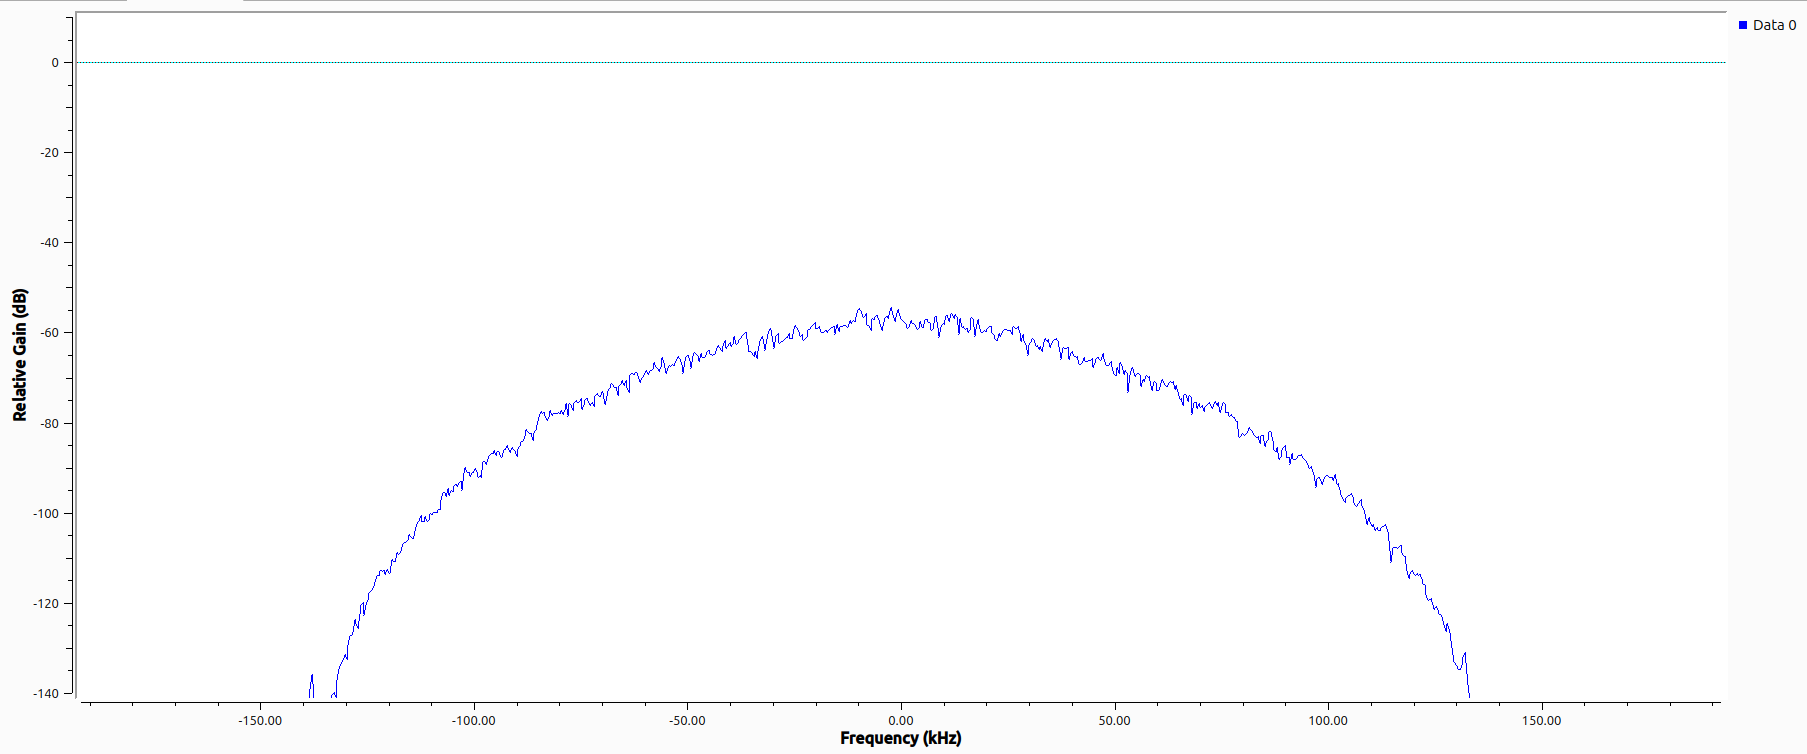
\includegraphics[width=0.7\textwidth]{fm_radio_user_lpf_spectrum.png}}}
	\caption{FM Radio LPF Spectrum}
	\label{fig::fm_radio_user_lpf_spectrum}
\end{figure}

\noindent Again, we note that the spectrum is roughly the same as our prior results, which are shown in Figure \ref{fig::fm_radio_lpf_spectrum}. Next, we capture the spectrum of the signal after demodulation, which is shown in Figure \ref{fig::fm_radio_user_demod_spectrum}.

\begin{figure}[H]
	\centerline{\fbox{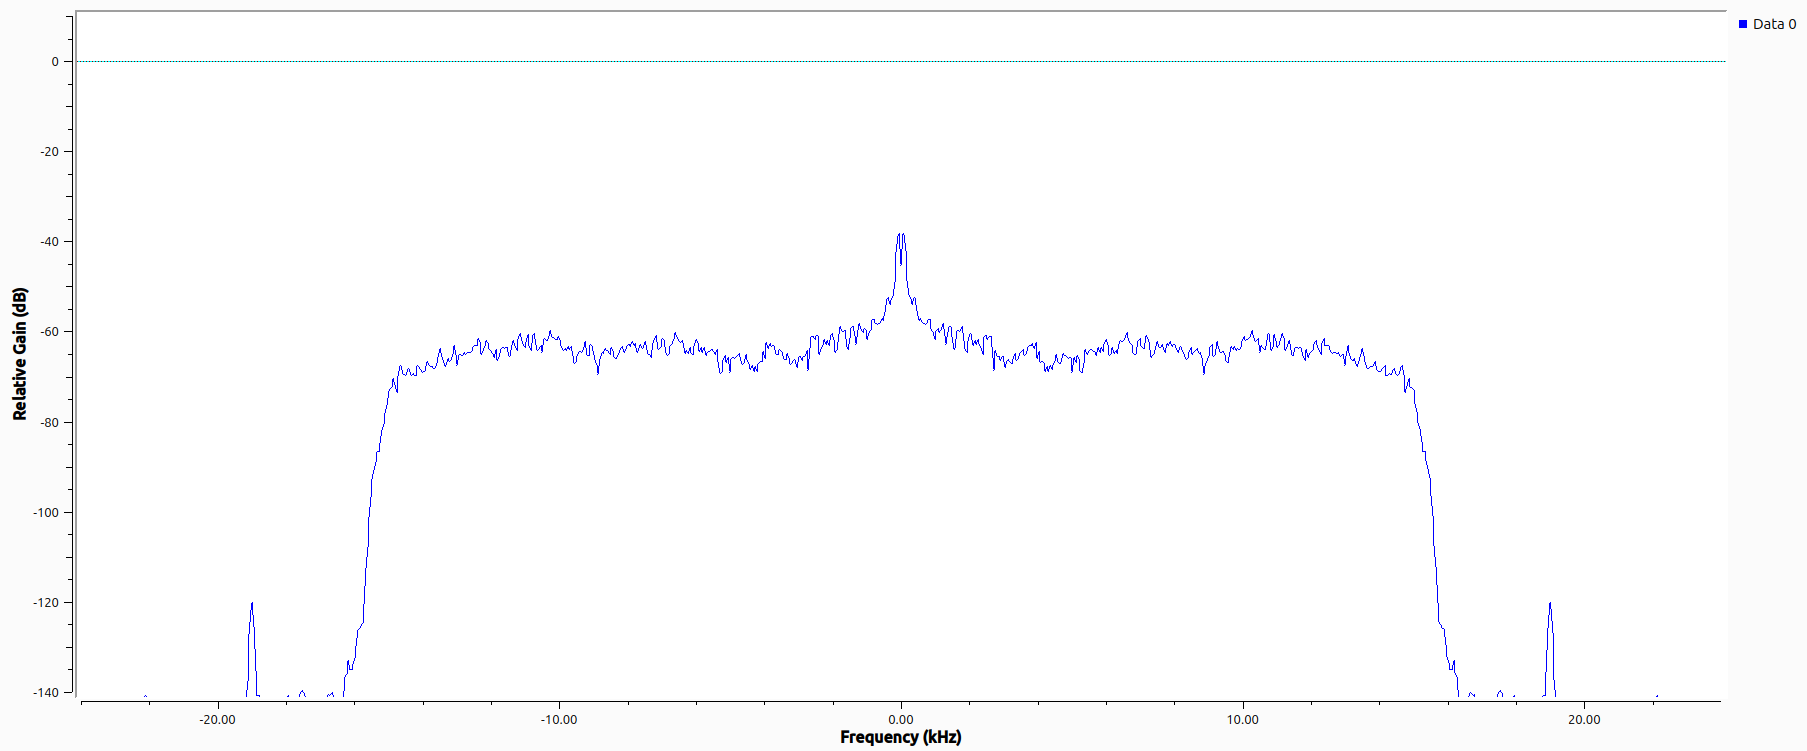
\includegraphics[width=0.7\textwidth]{fm_radio_user_demod_spectrum.png}}}
	\caption{Demodulated FM Signal Spectrum}
	\label{fig::fm_radio_user_demod_spectrum}
\end{figure}

\noindent Compared to the spectrum shown in Figure \ref{fig::fm_radio_demod_spectrum}, the demodulated signal spectrum does not have a gradual roll-off starting at DC. This is because the flowchart does not implement FM de-emphasis.

The updated flowchart shown in Figure \ref{fig::fm_radio_user_flowchart} contains the same decimation blocks as the flowchart shown in Figure \ref{fig::fm_radio_flowchart}. The first low-pass filter includes a decimate by 6, which results in a sample rate just greater than the bandwidth of the FM radio signal. The second filter decimates the demodulated signal output. This results in a signal with a sample rate of 48 kHz, exactly the rate that the audio sink needs.

The audio quality of the updated flowchart is comparable to that of the initial flowchart. However, a couple modifications would improve the audio quality. First, the flowchart has an RF bandwidth of 20 MHz. As discussed above, reducing the RF bandwidth, will improve the signal-to-noise ratio of the sampled signal. Another modification that would improve the audio quality is adding FM de-emphasis, which complements the FM pre-emphasis present in the transmitter. FM pre-emphasis amplifies the high frequency components of the signal before modulation to improve signal-to-noise ratio. FM de-emphasis inverts the frequency response of the pre-emphasis filter. We can add an FM de-emphasis block in GNU radio to implement the required de-emphasis filter.

\section{Questions}

In this section, we answer questions about AM modulation. Note that we cannot demodulate AM radio in the PlutoSDR, without additional hardware such as an upconverter. This is because the AM radio band (530 kHz - 1700 kHz) is outside of the Pluto's operating frequencies (70 MHz - 6 GHz). Car stereos, on the other hand, are specifically designed to receive signals in this band and do not require additional hardware.

Due to these deficiencies, we discuss the demodulation that we would perform if we had the additional hardware. The "AM Demod" block in GNU radio, is typically used to perform this demodulation. However, we can instead use a "Complex to Mag" block followed by a bandpass filter. Note that we use a band-pass filter instead of a low-pass filter to remove the carrier signal that is transmitted with the AM signal.
  
\section{Conclusion}
% Conclusions to the overall lab that discuss meaningful lessons learned and other takeaways from the assignment. (Important)

In this lab, we investigated analog demodulation with GNU radio. We specifically implemented GNU radio flowcharts to perform FM demodulation. In our first flowchart, we used the built-in FM demodulation block. Then, we examined the spectrum before and after demodulation. The output spectrum was distinct from the input spectrum because the demodulator returned the instantaneous frequency of the signal bandlimited to $\pm 15\ \text{kHz}$.

To get to the audio rate, we had to decimate the signal by a factor of 48. We performed this decimation in 2 stages. First, we decimated the signal by a factor of 6 to get a sampling rate of 384 kHz. This decimated rate was just large enough to represent the FM radio signal, which had a bandwidth of 200 kHz. In our first decimation stage, we used a filter with a cutoff frequency of 100 kHz instead of 192 kHz to eliminate any out-of-band noise prior to demodulation. Then, after demodulation, we decimated the resulting signal to match the rate of the audio sink. We were able to avoid using a rational resampler block because our sampling rate was a multiple of the audio rate. Avoiding unnecessary interpolation in the rational resampler block allowed us to eliminate any unnecessary processing.

The audio quality of our first flowchart was pretty good. However, the input SNR was degraded by the 20 MHz RF bandwidth. This bandwidth was larger than the sampling rate, which resulted in noise aliasing back into our spectrum. To improve our signal 	quality, we learned that we should reduce the RF bandwidth to a rate less than sampling rate and greater than the FM signal bandwidth.

In the input spectrum, we saw that the spectrum of the FM radio signal was about 200 kHz wide. To remove the out-of-band noise prior to FM demodulation, we processed the signal with a low-pass filter that had a 100 kHz cutoff frequency (200 kHz bandwidth) and a decimation rate of 6. We then passed the low-pass filter output into an FM demodulation block. This block measured the instantaneous frequency by computing the phase difference between adjacent samples. It then filtered the resulted signal with a 15 kHz cutoff frequency to remove noise outside of the audio band. Finally  

The spectrum 

- FM Radio spectrum about 200 kHz wide
- Filter signal before demodulation to remove out-of-band noise prior to demodulation
- Need to decimate demodulated signal to rate of audio sink.
- Can avoid using rational resampler block if our input sampling rate is a multiple of the audio sink rate.
- Limit RF bandwidth below the sampling rate to improve SNR.
- Replace FM demodulation block with quadrature demodulation block and low pass filter.
- Missing FM de-emphasis block
%\nocite{analog_devices_libiio_error}
%\bibliographystyle{IEEEtran}
%\bibliography{sources}{}
%\bibliographystyle{ieeetr}
	
\end{document}